\documentclass{article}
\usepackage[utf8]{inputenc}

\usepackage{amsfonts}
\usepackage{amssymb}
\usepackage{amsmath}
\usepackage{amsthm}
\usepackage{enumitem}

\usepackage{bbold}
\usepackage{bm}
\usepackage{graphicx}
\usepackage{color}
\usepackage{hyperref}
\usepackage[margin=2.5cm]{geometry}

\begin{document}


% ==============================================================================

\title{\Large{INFO8006: Project 2 - Report}}
\vspace{1cm}
\author{\small{\bf HOGGE Louis - s192814} \\ \small{\bf LECLERC Emilien - s190701}}

\maketitle

% ==============================================================================

\section{Problem statement}

\begin{enumerate}[label=\alph*.,leftmargin=*]
    \item
    \begin{itemize}
        \item Let a state of the game be a pair s = (g, p) , where g is the current grid that comports the postion of Pacman, the Ghost, the walls, the food dots and the cells that are not walls directly next to pacman and the ghost. p is the player to play next.
        \\
        \\
        \textbf{Initial state} s0 = (g, 0) where g depends on the layout. 
        \item \textbf{Player function} player(s = (g, p)) = p.
        \item \textbf{Actions}  An action is represented by a legal move to a cell, that is not a wall, next to the player in the grid. Then, the set of possible actions is actions(s = (g, p)) = \{North, South, West, East, Stop if these moves are legal i.e. if they don't lead to a walll\}.
        \item \textbf{Transition model} For an action a $\in$ actions(s),
s' = result(s = (g, p), a) = (g', p + 1 mod 2). g' is the next grid diposition.
        \item \textbf{Terminal test} terminal(s) is true if Pacman dead or all foods eaten, false otherwise.
        \item \textbf{Utility function} utility(s = (g, p = Pacman)) = -\#time steps + 10*\#number of eaten food dots + (-500 if \#losing end) + (500 if \#winning end) where \#time step is the number of moves that Pacman has done during the game, \#losing end = 1 if Pacman and the ghost are at the same position at the same time and it lefts at least one food dot in the grid at an other position, 0 otherwise, \#winning end = 1 if there is no food dot left in the grid, 0 otherwise.
    \end{itemize}
    \item If the game was a zero-sum game, we would define utility(s, p) for p = Ghost as utility(s, p) = 1 if  \#losing end = 1 i.e. Pacman Lose, -1 if \#winning end = 1 i.e. Pacman Win.

\end{enumerate}

\section{Implementation}

\begin{enumerate}[label=\alph*.,leftmargin=*]
    \item Yes, if the tree generated by Minimax is finite i.e. if Pacman doesn't enter in a cycle. The tree is finite if it exists a valid path to access each food dots. If the ghost prevent Pacman from being able to access a food dot, Pacman could enter in a cycle.
    \\
    \\
    Going through a cycle (i.e., going back to an already visited state s) will only increase the \#time steps. In a zero-sum game the score only depends on \#winning end and  \#losing end so there is no advantage in going through a cycle.
    \\
    \\
    To guarantee the completeness of Minimax we need to limit the maximum depth of the tree generated. As we know that cycles are useless, the best way to limit the tree's depth is to to limit it to the maximum number of differents states of the game.
    \\
    \\
    \item minimax(state, agent, depth) =
    \\
    \begin{equation}
    \begin{cases}
      Utility(s) & \text{if Terminal-Test(s}) \\
      max_{a \in Action(s)}minimax(Result(s,a)) & \text{if Player(s) = MAX}\\
      min_{a \in Action(s)}minimax(Result(s,a)) & \text{if Player(s) = MIN}
    \end{cases}
  \end{equation}
    \item hminimax0(state, agent, depth) =
    \\
    \begin{equation}
    \begin{cases}
      eval(s) & \text{if Cutoff-Test(s,d)}) \\
      max_{a \in Action(s)}hminimax0(Result(s,a)) & \text{if Player(s) = MAX}\\
      min_{a \in Action(s)}hminimax0(Result(s,a)) & \text{if Player(s) = MIN}
    \end{cases}
  \end{equation}
    \\
    hminimax1(state, agent, depth, initial\_numfood) =
    \\
    \begin{equation}
    \begin{cases}
      eval(s) & \text{if Cutoff-Test(s,d)}) \\
      max_{a \in Action(s)}hminimax1(Result(s,a)) & \text{if Player(s) = MAX}\\
      min_{a \in Action(s)}hminimax1(Result(s,a)) & \text{if Player(s) = MIN}
    \end{cases}
  \end{equation}
\\
hminimax2(state, agent, depth, depth\_N, depth\_S, depth\_W, depth\_E) =
    \\
    \begin{equation}
    \begin{cases}
      eval(s) & \text{if Cutoff-Test(s,d)}) \\
      max_{a \in Action(s)}hminimax2(Result(s,a)) & \text{if Player(s) = MAX}\\
      min_{a \in Action(s)}hminimax2(Result(s,a)) & \text{if Player(s) = MIN}
    \end{cases}
  \end{equation}
\\
hminimax0 : This is our most efficient one that use the A-star algorithm to find the succesors of pacman. The cutoff only stops the recursive in function of his depth and evaluate the score added to an heuristic that calculates the distance between pacman and the nearest dot.
\\
\\
hminimax1 : The cutoff stops the recursive in fonction of his depth, but the maximal depth decreases while pacman eat food dots. For the evaluation function, when a food is eaten it returns the score added to the depth of this recursive, when the maximal depth is passed, it returns the score in function of the distance between pacman and the nearest food dot.
\\
\\
hminimax2 : The same evaluation function as hminimax1 using the distance between pacman and the food dots and a cutoff when the maximal depth is passed. But the maximal depth is calculated in function of the position of the ghost, in order avoid expanding nodes that are behind the ghost (in the perspective of pacman).

\end{enumerate}

\section{Experiment}

\begin{enumerate}[label=\alph*.,leftmargin=*]
    \item Results are at the end of the report.
    \begin{figure}[!hb]
    \centering 
    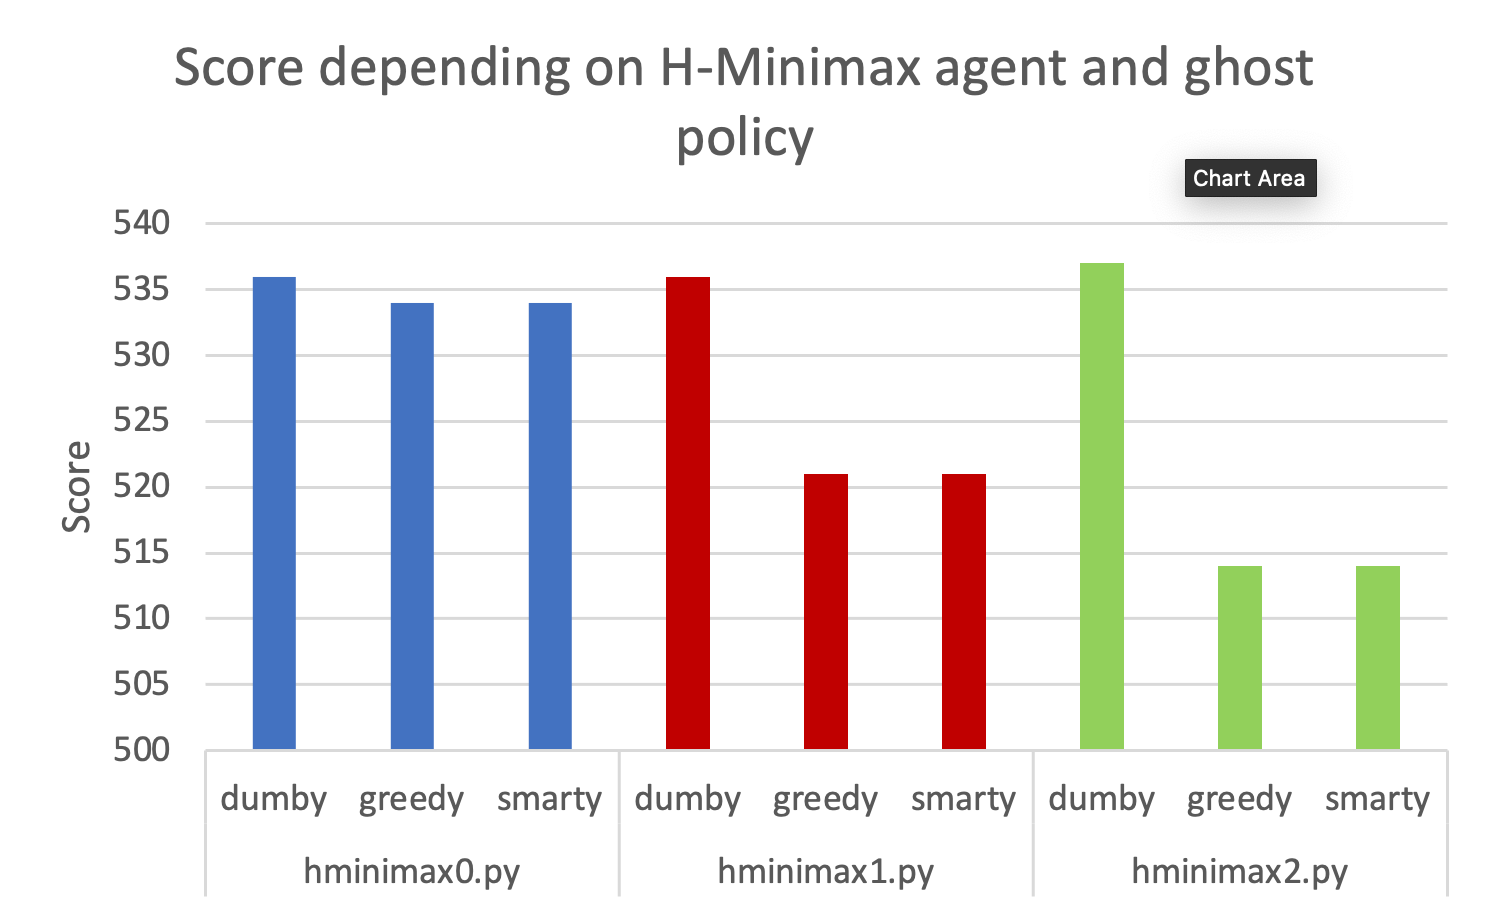
\includegraphics[scale = 0.5]{score}
    \end{figure}
    
    \begin{figure}[!hb]
    \centering 
    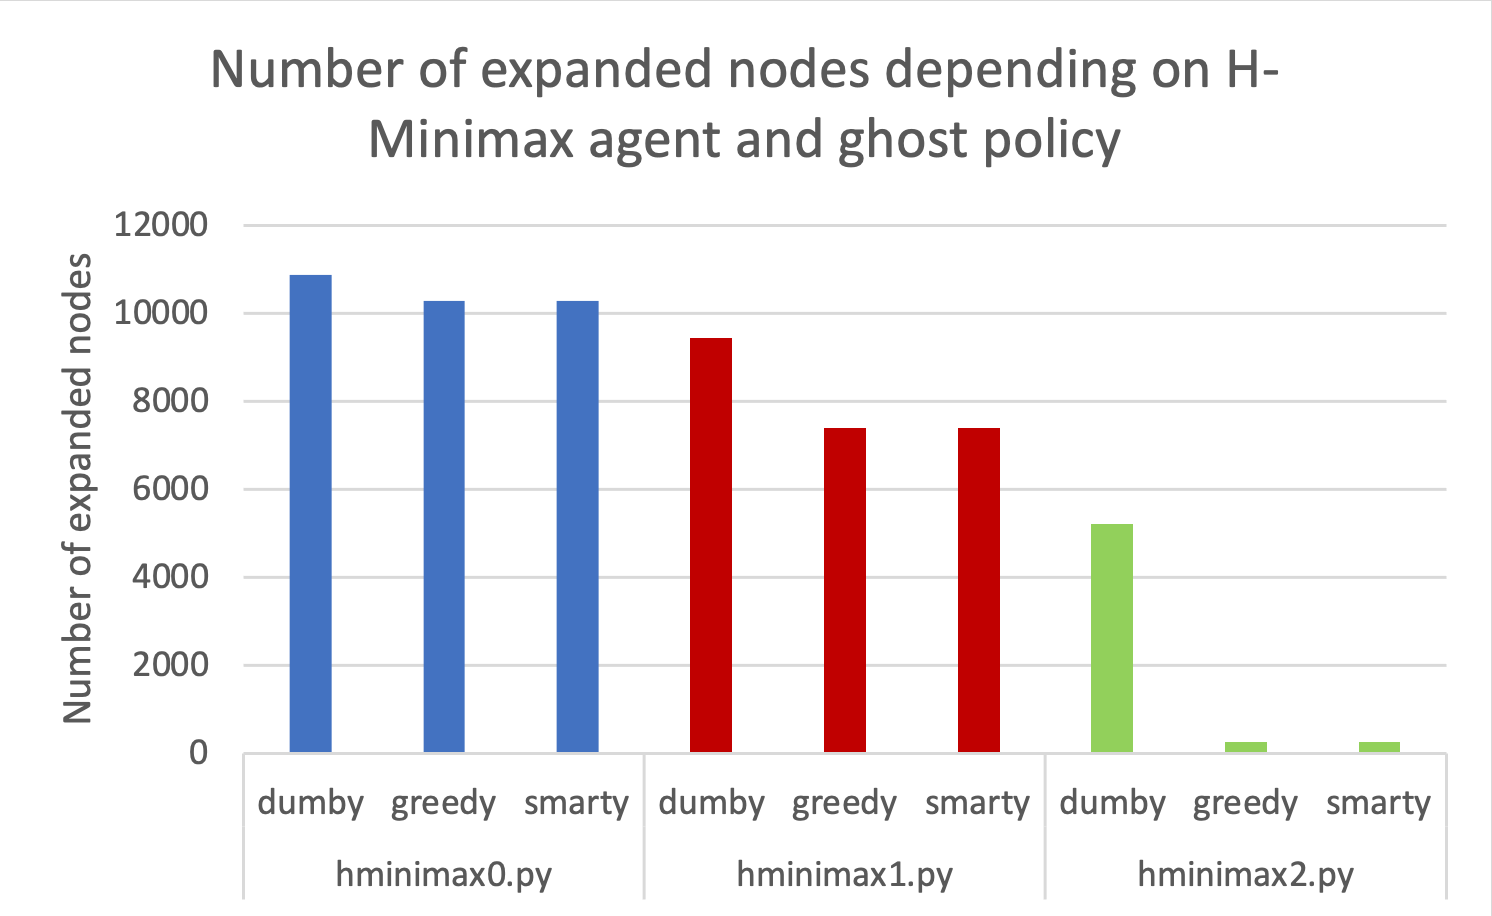
\includegraphics[scale = 0.5]{nodes}
    \end{figure}
    
    \begin{figure}[ht]
    \centering 
    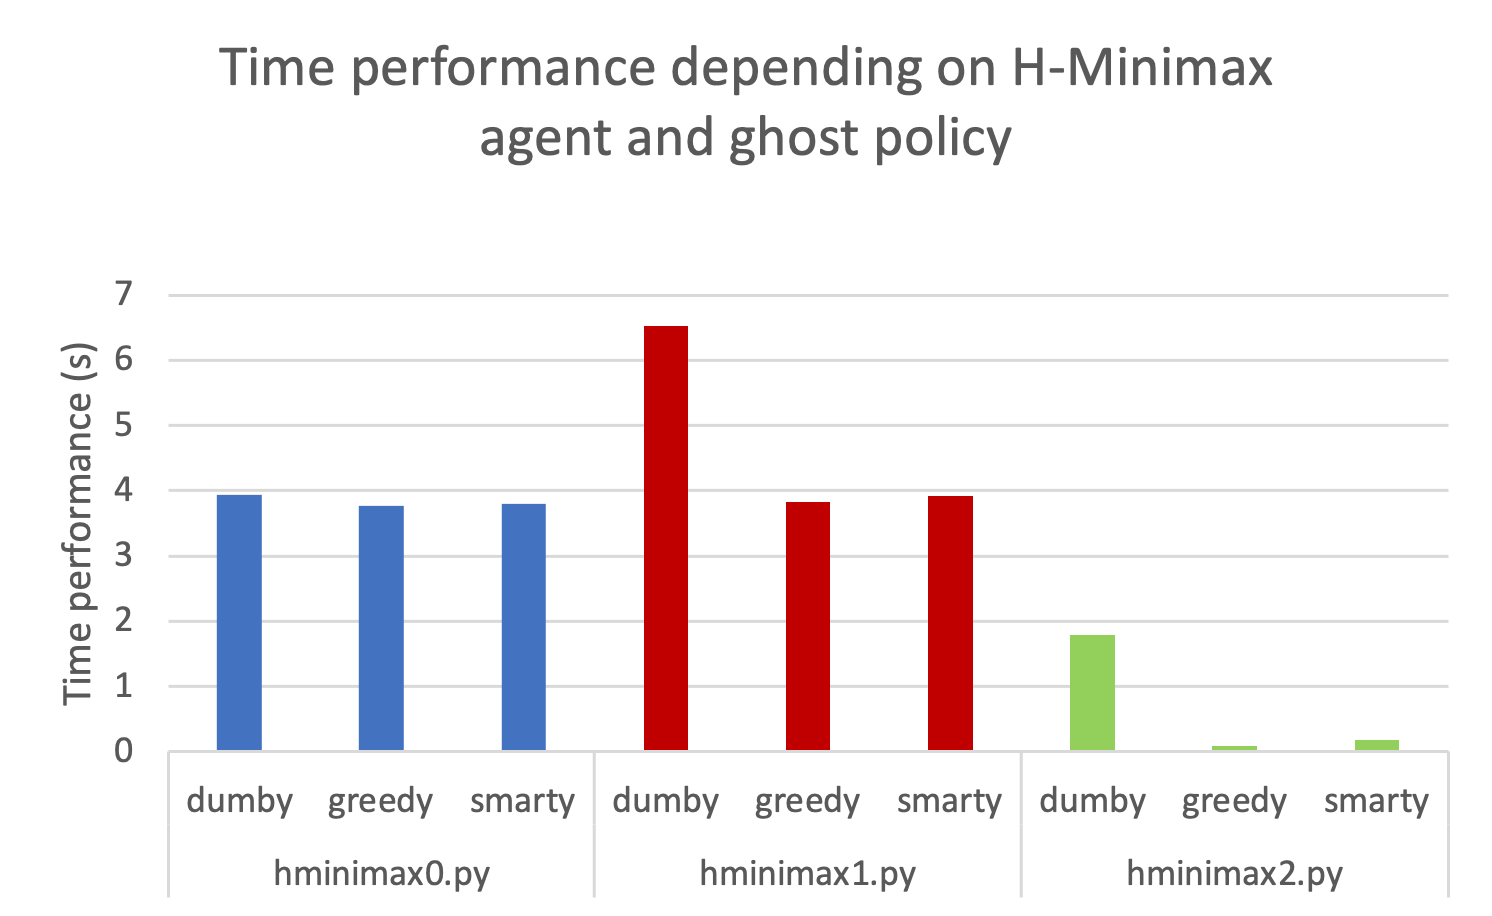
\includegraphics[scale = 0.5]{time}
    \end{figure}
   
    \item We can see that hminimax0 is globally the best  because it uses the A-star algorithm to generate the succesors of pacman and find a pretty good one. But it expands a lot of nodes like hminimax1. Indeed, the two uses a maximal depth in minimax for the cutoff. However, hminimax1 explores slightly less nodes, because it adjusts his maximal depth in function of the number of food dots left and operate a cutoff directly if a food his eaten.
The third one, hminimax2, finds a score better than the others with a dumby ghost. But like hminimax1, the score with a greedy or a smarty ghost is less effective.
hminimax2 is the fastest with a very small number of nodes expanded because minimax avoid expanding nodes that are behind the ghost (in the perspective of pacman).
\end{enumerate}



% ==============================================================================

\end{document}
